\documentclass[thesis-solanki.tex]{subfiles}


\begin{document}

\chapter{Prototype 2.1}{\label{proto2.1}}

\section{About this chapter}
This chapter attempts to infuse the generic methodology from \ref{proto1} in a current \progLang{Prolog} implementation \cite{prolog-lib}
and make the unification ``monadic''.

\section{How prolog-0.2.0.1 works}

As described in the previous chapter about extending languages to incorporate functionality, this prototype applies the procedure to the
eDSL in \cite{prolog-lib}.

The original abstract syntax used by the library,
\begin{code-list}[h]
\begin{minted}[linenos]{haskell}

data VariableName = VariableName Int String
      deriving (Eq, Data, Typeable, Ord)

type Atom         = String

data Term = Struct Atom [Term]
          | Var VariableName
          | Wildcard -- Don't cares
          | Cut Int
      deriving (Eq, Data, Typeable)

data Clause = Clause { lhs :: Term, rhs_ :: [Goal] }
            | ClauseFn { lhs :: Term, fn :: [Term] -> [Goal] }
      deriving (Data, Typeable)

type Goal         = Term
type Program      = [Clause]
\end{minted}
\caption{Current Language Implementation}
\label{tab:currlangimpl}
\end{code-list}

From the Figure~\ref{tab:currlangimpl} we will focus on the \textit{Term} since the others just add wrappers around expressions which can
be created by it. The above language suffers from most of the problems discussed in the previous chapter. The above is used to construct
\progLang{Prolog} ``terms'' which are of a ``single type''.


The implementation consists of components that one would find in a Language Processing System \ref{fig:A language-processing system},

\begin{figure}[th]
\centering
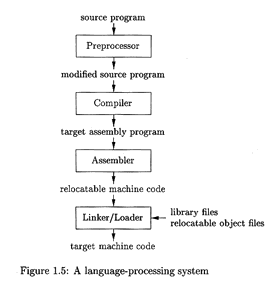
\includegraphics[scale = 0.7]{Language_Processing_System.png}
\caption{A language-processing system \cite{Aho:1986:CPT:6448}}
\label{fig:A language-processing system}
\end{figure}

specifically speaking, parts of a compiler \ref{fig:Phases of Compiler},

\begin{figure}[th]
\centering
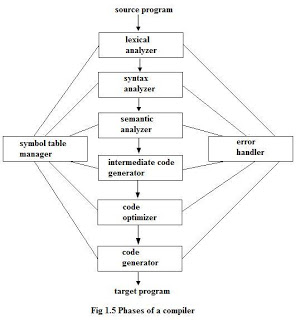
\includegraphics[scale = 0.7]{Phases_of_compiler.jpg}
\caption{Phases of Compiler \cite{Aho:1986:CPT:6448}}
\label{fig:Phases of Compiler}
\end{figure}

The architecture for a compiler as described in \ref{fig:Phases of Compiler} would not be needed since \progLang{Haskell} provides most of
them. Nonetheless, the library has the following major components,

\begin{enumerate}
\item Syntax, defining the language.

\item Database, to create a storage for the expressions.

\item Parser.

\item Interpreter.

\item Unifier.

\item Read-Eval-Print Loop(REPL). 
\end{enumerate}

To prove the modularity of the approach for language modification and monadic unification only the abstract syntax and unifier will be
customized.


\clearpage
\section{What we do in this prototype?}
In the first prototype we just did unification of two terms not query resolution.

We do complete \progLang{Prolog} query resolution like stuff.

\ref{proto1} provides a generic procedure / methodology to convert a language into monadic unifiable form

\clearpage
\section{Current implementation (prolog-0.2.0.1)}

Beginning with language from Figure~\ref{tab:currlangimpl} is transformed into an isomorphically equivalent grammar described in 
Figure~\ref{tab:flatgrp0201}

\begin{code-list}[h]
\begin{minted}[linenos]{haskell}
data FTS a = FS Atom [a] | FV VariableName | FW | FC Int
                          deriving (Show, Eq, Typeable, Ord)

newtype Prolog = P (Fix FTS) deriving (Eq, Show, Ord, Typeable)

unP :: Prolog -> Fix FTS
unP (P x) = x

instance Functor (FTS) where
  fmap              = T.fmapDefault

instance Foldable (FTS) where
  foldMap             = T.foldMapDefault

instance Traversable (FTS) where
    traverse f (FS atom xs)      =   FS atom <$> sequenceA (Prelude.map f xs)
    traverse _ (FV v)          =   pure (FV v)
    traverse _ FW         =   pure (FW)
    traverse _ (FC i)          =   pure (FC i)

instance Unifiable (FTS) where
  zipMatch (FS al ls) (FS ar rs) = 
    if (al == ar) && (length ls == length rs) 
      then FS al <$> pairWith (\l r -> Right (l,r)) ls rs     
      else Nothing
  zipMatch FW _ = Just FW
  zipMatch _ FW = Just FW
  zipMatch (FC i1) (FC i2) = if (i1 == i2) 
    then Just (FC i1) 
    else Nothing

instance Applicative (FTS) where
  pure x                  =   FS "" [x] 
  _         <*>   FW    =   FW
  _       <*>   (FC i)     =   FC i
  _       <*>   (FV v)     = (FV v)
  (FS a fs) <*> (FS b xs)   = FS (a ++ b) [f x | f <- fs, x <- xs]

\end{minted}
\caption{Flattened (non-recursive) grammar}
\label{tab:flatgrp0201}
\end{code-list}

\clearpage

The current unification uses basic pattern matching to unify the terms. 

The process returns a Unifier,
\begin{code-list}[h]
\begin{minted}[linenos]{haskell}
type Unifier      = [Substitution]
type Substitution = (VariableName, Term)
\end{minted}
\caption{prolog-0.2.0.1 Unifier}
\label{tab:prlg0201unifier}
\end{code-list}
Figure~\ref{tab:prlg0201unifier} shows the result type. The instances are created to open up the language and make it compatible with the
unification library \cite{prolog-lib}.

\clearpage

Coming back to the unification itself shown in Figure~\ref{tab:prlg0201unification}. Each language expression is matched based on its 
structure.
  
\begin{code-list}[h]
\begin{minted}[linenos]{haskell}
unify, unify_with_occurs_check :: MonadPlus m => Term -> Term
-> m Unifier

unify = fix unify'

unify_with_occurs_check =
   fix $ \self t1 t2 -> if (t1 `occursIn` t2 || t2 `occursIn` t1)
                           then fail "occurs check"
                           else unify' self t1 t2
 where
   occursIn t = everything (||) (mkQ False (==t))

unify' :: MonadPlus m => (Term -> Term -> m Unifier) -> Term ->
Term -> m [(VariableName, Term)]

-- If either of the terms are don't cares then no unifiers exist
unify' _ Wildcard _ = return []
unify' _ _ Wildcard = return []

-- If one is a variable then equate the term to its value which
-- forms the unifier
unify' _ (Var v) t  = return [(v,t)]
unify' _ t (Var v)  = return [(v,t)]

-- Match the names and the length of their parameter list and
-- then match the elements of list one by one.
unify' self (Struct a1 ts1) (Struct a2 ts2)
            | a1 == a2 && same length ts1 ts2 =
            unifyList self (zip ts1 ts2)

unify' _ _ _ = mzero

same :: Eq b => (a -> b) -> a -> a -> Bool
same f x y = f x == f y

-- Match the elements of each of the tuples in the list.
unifyList :: Monad m => (Term -> Term -> m Unifier) ->
[(Term, Term)] -> m Unifier
unifyList _ [] = return []
unifyList unify ((x,y):xys) = do
   u  <- unify x y
   u' <- unifyList unify (Prelude.map (both (apply u)) xys)
   return (u++u')
\end{minted} 
\caption{prolog-0.2.0.1 Unification}
\label{tab:prlg0201unification}
\end{code-list}

The issue with the current appraoch is the rigidity of the procedure. Any language modification will cause a ripple effect across the 
system. As described in Chapter~\ref{proto1}, the advantages of \textit{functorizing} language hold in this implementation as well.

\clearpage
\section{Modifications}
The resulting language is not far from what we did in \ref{proto1} apart from the fact that the \textit{Term} expressions are encapsulated
to form \textit{Clauses} which in turn form a \textit{Program}.

Moreover, the required instances make the language compatible with the unification procedure.

\begin{minted}[linenos]{haskell}
data FTS a = FS Atom [a] | FV VariableName | FW | FC Int
                          deriving (Show, Eq, Typeable, Ord)

newtype Prolog = P (Fix FTS) deriving (Eq, Show, Ord, Typeable)

unP :: Prolog -> Fix FTS
unP (P x) = x

instance Functor (FTS) where
  fmap              = T.fmapDefault

instance Foldable (FTS) where
  foldMap             = T.foldMapDefault

instance Traversable (FTS) where
    traverse f (FS atom xs)      =   FS atom <$>
    sequenceA (Prelude.map f xs)
    traverse _ (FV v)          =   pure (FV v)
    traverse _ FW         =   pure (FW)
    traverse _ (FC i)          =   pure (FC i)

instance Unifiable (FTS) where
  zipMatch (FS al ls) (FS ar rs) =
    if (al == ar) && (length ls == length rs)
      then FS al <$> pairWith (\l r -> Right (l,r)) ls rs
      else Nothing
  zipMatch FW _ = Just FW
  zipMatch _ FW = Just FW
  zipMatch (FC i1) (FC i2) = if (i1 == i2)
    then Just (FC i1)
    else Nothing

instance Applicative (FTS) where
  pure x                  =   FS "" [x]
  _         <*>   FW    =   FW
  _       <*>   (FC i)     =   FC i
  _       <*>   (FV v)     = (FV v)
  (FS a fs) <*> (FS b xs)   = FS (a ++ b) [f x | f <- fs, x <- xs]
\end{minted}

Aditionally helper functions for converting expressions between the two domains and translation to \textit{UTerm}.

To solve the issue of infinitely deep language expressions, we find the fixed point of the expression. The unification function provided by 
\cite{prolog-lib} is not very \progLang{Prolog} like in nature and certain adjustments need to be made. 
\begin{enumerate}
\item Extracting variable and creating dictionaries.

\item Converting to UTerms and back
\end{enumerate}

\begin{minted}[linenos]{haskell}

termFlattener :: Term -> Fix FTS
termFlattener (Var v)           =   DFF.Fix $ FV v
termFlattener (Wildcard)        =   DFF.Fix FW
termFlattener (Cut i)           =   DFF.Fix $ FC i
termFlattener (Struct a xs)     =   DFF.Fix $ FS a (Prelude.map termFlattener xs)

unFlatten :: Fix FTS -> Term
unFlatten (DFF.Fix (FV v))      =   Var v
unFlatten (DFF.Fix FW)          =   Wildcard
unFlatten (DFF.Fix (FC i))      =   Cut i
unFlatten (DFF.Fix (FS a xs))   =   Struct a (Prelude.map unFlatten xs)


variableExtractor :: Fix FTS -> [Fix FTS]
variableExtractor (Fix x) = case x of
  (FS _ xs)   ->  Prelude.concat $ Prelude.map variableExtractor xs
  (FV v)     ->  [Fix $ FV v]
  _       ->  []

variableNameExtractor :: Fix FTS -> [VariableName]
variableNameExtractor (Fix x) = case x of
  (FS _ xs) -> Prelude.concat $ Prelude.map variableNameExtractor xs
  (FV v)     -> [v]
  _         -> []

variableSet :: [Fix FTS] -> S.Set (Fix FTS)
variableSet a = S.fromList a

variableNameSet :: [VariableName] -> S.Set (VariableName)
variableNameSet a = S.fromList a

varsToDictM :: (Ord a, Unifiable t) =>
    S.Set a -> ST.STBinding s (Map a (ST.STVar s t))
varsToDictM set = foldrM addElt Map.empty set where
  addElt sv dict = do
    iv <- freeVar
    return $! Map.insert sv iv dict


uTermify
  :: Map VariableName (ST.STVar s (FTS))
  -> UTerm FTS (ST.STVar s (FTS))
  -> UTerm FTS (ST.STVar s (FTS))
uTermify varMap ux = case ux of
  UT.UVar _             -> ux
  UT.UTerm (FV v)       -> maybe (error "bad map") UT.UVar $ Map.lookup v varMap
 -- UT.UTerm t            -> UT.UTerm $! fmap (uTermify varMap) t
  UT.UTerm (FS a xs)    -> UT.UTerm $ FS a $! fmap (uTermify varMap) xs
  UT.UTerm (FW)         -> UT.UTerm FW
  UT.UTerm (FC i)       -> UT.UTerm (FC i)

translateToUTerm ::
    Fix FTS -> ST.STBinding s
            (UT.UTerm (FTS) (ST.STVar s (FTS)),
             Map VariableName (ST.STVar s (FTS)))
translateToUTerm e1Term = do
  let vs = variableNameSet $ variableNameExtractor e1Term
  varMap <- varsToDictM vs
  let t2 = uTermify varMap . unfreeze $ e1Term
  return (t2,varMap)


-- | vTermify recursively converts @UVar x@ into @UTerm (VarA x).
-- This is a subroutine of @ translateFromUTerm @.  The resulting
-- term has no (UVar x) subterms.

vTermify :: Map Int VariableName ->
            UT.UTerm (FTS) (ST.STVar s (FTS)) ->
            UT.UTerm (FTS) (ST.STVar s (FTS))
vTermify dict t1 = case t1 of
  UT.UVar x  -> maybe (error "logic") (UT.UTerm . FV) $ Map.lookup (UT.getVarID x) dict
  UT.UTerm r ->
    case r of
      FV iv   -> t1
      _       -> UT.UTerm . fmap (vTermify dict) $ r

translateFromUTerm ::
    Map VariableName (ST.STVar s (FTS)) ->
    UT.UTerm (FTS) (ST.STVar s (FTS)) -> Prolog
translateFromUTerm dict uTerm =
  P .  maybe (error "Logic") id . freeze . vTermify varIdDict $ uTerm where
    forKV dict initial fn = Map.foldlWithKey' (\a k v -> fn k v a) initial dict
    varIdDict = forKV dict Map.empty $ \ k v -> Map.insert (UT.getVarID v) k


-- | Unify two (E1 a) terms resulting in maybe a dictionary
-- of variable bindings (to terms).
--
-- NB !!!!
-- The current interface assumes that the variables in t1 and t2 are
-- disjoint.  This is likely a mistake that needs fixing

unifyTerms :: Fix FTS -> Fix FTS -> Maybe (Map VariableName (Prolog))
unifyTerms t1 t2 = ST.runSTBinding $ do
  answer <- runExceptT $ unifyTermsX t1 t2
  return $! either (const Nothing) Just answer

-- | Unify two (E1 a) terms resulting in maybe a dictionary
-- of variable bindings (to terms).
--
-- This routine works in the unification monad

unifyTermsX ::
    (Fix FTS) -> (Fix FTS) ->
    ExceptT  (UT.UFailure (FTS) (ST.STVar s (FTS)))
        (ST.STBinding s)
        (Map VariableName (Prolog))
unifyTermsX t1 t2 = do
    (x1,d1) <- lift . translateToUTerm $ t1
    (x2,d2) <- lift . translateToUTerm $ t2
    _ <- U.unify x1 x2
    makeDicts $ (d1,d2)

mapWithKeyM :: (Ord k,Applicative m,Monad m)
               => (k -> a -> m b) -> Map k a -> m (Map k b)
mapWithKeyM = Map.traverseWithKey


makeDict ::
            Map VariableName (ST.STVar s (FTS)) -> ST.STBinding s (Map VariableName (Prolog))
makeDict sVarDict =
    flip mapWithKeyM sVarDict $ \ _ -> \ iKey -> do
        Just xx <- UT.lookupVar $ iKey
        return $! (translateFromUTerm sVarDict) xx


-- | recover the bindings for the variables of the two terms
-- unified from the monad.

makeDicts ::
    (Map VariableName (ST.STVar s (FTS)), Map VariableName (ST.STVar s (FTS))) ->
    ExceptT  (UT.UFailure (FTS) (ST.STVar s (FTS)))
    (ST.STBinding s) (Map VariableName (Prolog))
makeDicts (svDict1, svDict2) = do
  let svDict3 = (svDict1 `Map.union` svDict2)
  let ivs = Prelude.map UT.UVar . Map.elems $ svDict3
  applyBindingsAll ivs
  -- the interface below is dangerous because Map.union is left-biased.
  -- variables that are duplicated across terms may have different
  -- bindings because `translateToUTerm` is run separately on each
  -- term.
  lift . makeDict $ svDict3
\end{minted}

Take original expressions flatten fix convert unify
run it STBinding monad to extract substitutions.

\begin{minted}[linenos]{haskell}
monadicUnification :: (BindingMonad FTS (STVar s FTS)
(ST.STBinding s))
=> (forall s. ((Fix FTS) -> (Fix FTS) ->
  ErrorT (UT.UFailure (FTS) (ST.STVar s (FTS)))
           (ST.STBinding s) (UT.UTerm (FTS) (ST.STVar s (FTS)),
            Map VariableName (ST.STVar s (FTS)))))
monadicUnification t1 t2 = do
--  let
--    t1f = termFlattener t1
--    t2f = termFlattener t2
  (x1,d1) <- lift . translateToUTerm $ t1
  (x2,d2) <- lift . translateToUTerm $ t2
  x3 <- U.unify x1 x2
  --get state from somehwere, state -> dict
  return $! (x3, d1 `Map.union` d2)


goUnify ::
  (forall s. (BindingMonad FTS (STVar s FTS) (ST.STBinding s))
  =>
      (ErrorT
          (UT.UFailure FTS (ST.STVar s FTS))
          (ST.STBinding s)
          (UT.UTerm FTS (ST.STVar s FTS),
             Map VariableName (ST.STVar s FTS)))
     )
  -> [(VariableName, Prolog)]
goUnify test = ST.runSTBinding $ do
  answer <- runErrorT $ test --ERROR
  case answer of
    (Left _)            -> return []
    (Right (_, dict))   -> f1 dict


f1 ::
  (BindingMonad FTS (STVar s FTS) (ST.STBinding s))
  => (forall s. Map VariableName (STVar s FTS)
      -> (ST.STBinding s [(VariableName, Prolog)])
     )
f1 dict = do
  let ld1 = Map.toList dict
  ld2 <- Control.Monad.Error.sequence
  [ v1 | (k,v) <- ld1, let v1 = UT.lookupVar v]
  let ld3 = [ (k,v) | ((k,_),Just v) <- ld1 `zip` ld2]
      ld4 = [ (k,v) | (k,v2) <- ld3,
      let v = translateFromUTerm dict v2 ]
  return ld4
  unifierConvertor :: [(VariableName, Prolog)] -> Unifier
  unifierConvertor xs = Prelude.map (\(v, p) -> (v, (unFlatten $ unP $ p))) xs

unify :: MonadPlus m => Term -> Term -> m Unifier
unify t1 t2 = unifierConvertor (goUnify (monadicUnification (termFlattener t1) (termFlattener t2)))

\end{minted}



\section{Results}

It works,



\section{Chapter Recap}


\end{document}
